\documentclass[a4paper, UTF8,twoside]{ctexart}

\usepackage{ref/main}%在这里放置需要的宏包,并设置部分所需内容

\begin{document}

    \pagestyle{empty}%不要页眉页脚
    
    \begin{titlepage}
        \heiti
        \vspace*{64pt}
        \begin{center}
            
            \begin{figure}
                \centering
                
\includegraphics[width=1.0\textwidth]{graphic/0.jpg} %1.jpg是图片文件的相对路径
                \label{img} %此处的label相当于一个图片的专属标志,目的是方便上下文的引用
            \end{figure}
    
            \fontsize{48pt}{0}{\kaishu  机械设计基础}\\
            \vspace*{100pt}
        
            \LARGE 题目\ \ \underline{\makebox[200pt]{ 机械设计基础说明书 }}\\
            \LARGE 作者\ \ \underline{\makebox[200pt]{  }}\\
            \LARGE 学号\ \ \underline{\makebox[200pt]{ 0617104 }}\\
            \LARGE 学院\ \ \underline{\makebox[200pt]{材料科学与技术学院}}\\
            \LARGE 联系方式\ \ \underline{\makebox[200pt]{  }}\\
            \LARGE 指导老师\ \ \underline{\makebox[200pt]{  }}
            \vspace*{120pt}
    
            \LARGE 时间 \ \ \makebox[200pt]{ XX年XX月 }
    
        \end{center}
    \end{titlepage}

    %\maketitle
    \tableofcontents
    \zihao{-4}
    \thispagestyle{empty}%页脚不要页码
    %“目录”两个字的样式与section的样式一致,默认居中,故将设置section标题居左放置在生成目录后

    %%%%正文开始,页脚有页码
    \cfoot{\zihao{-5}第 \ \thepage \ 页 }
    %%%%lastpage为末页标签
    %正文
    \zihao{5}
    \pagenumbering{arabic}%页码使用阿拉伯数字
    \setcounter{page}{0}  %重新设置页码计数
    \pagestyle{fancy}

    \section{设计任务书}
\subsection{设计题目}
设计一级斜齿圆柱齿轮减速器\cite{于明礼}
\begin{figure}[h]
    \centering
    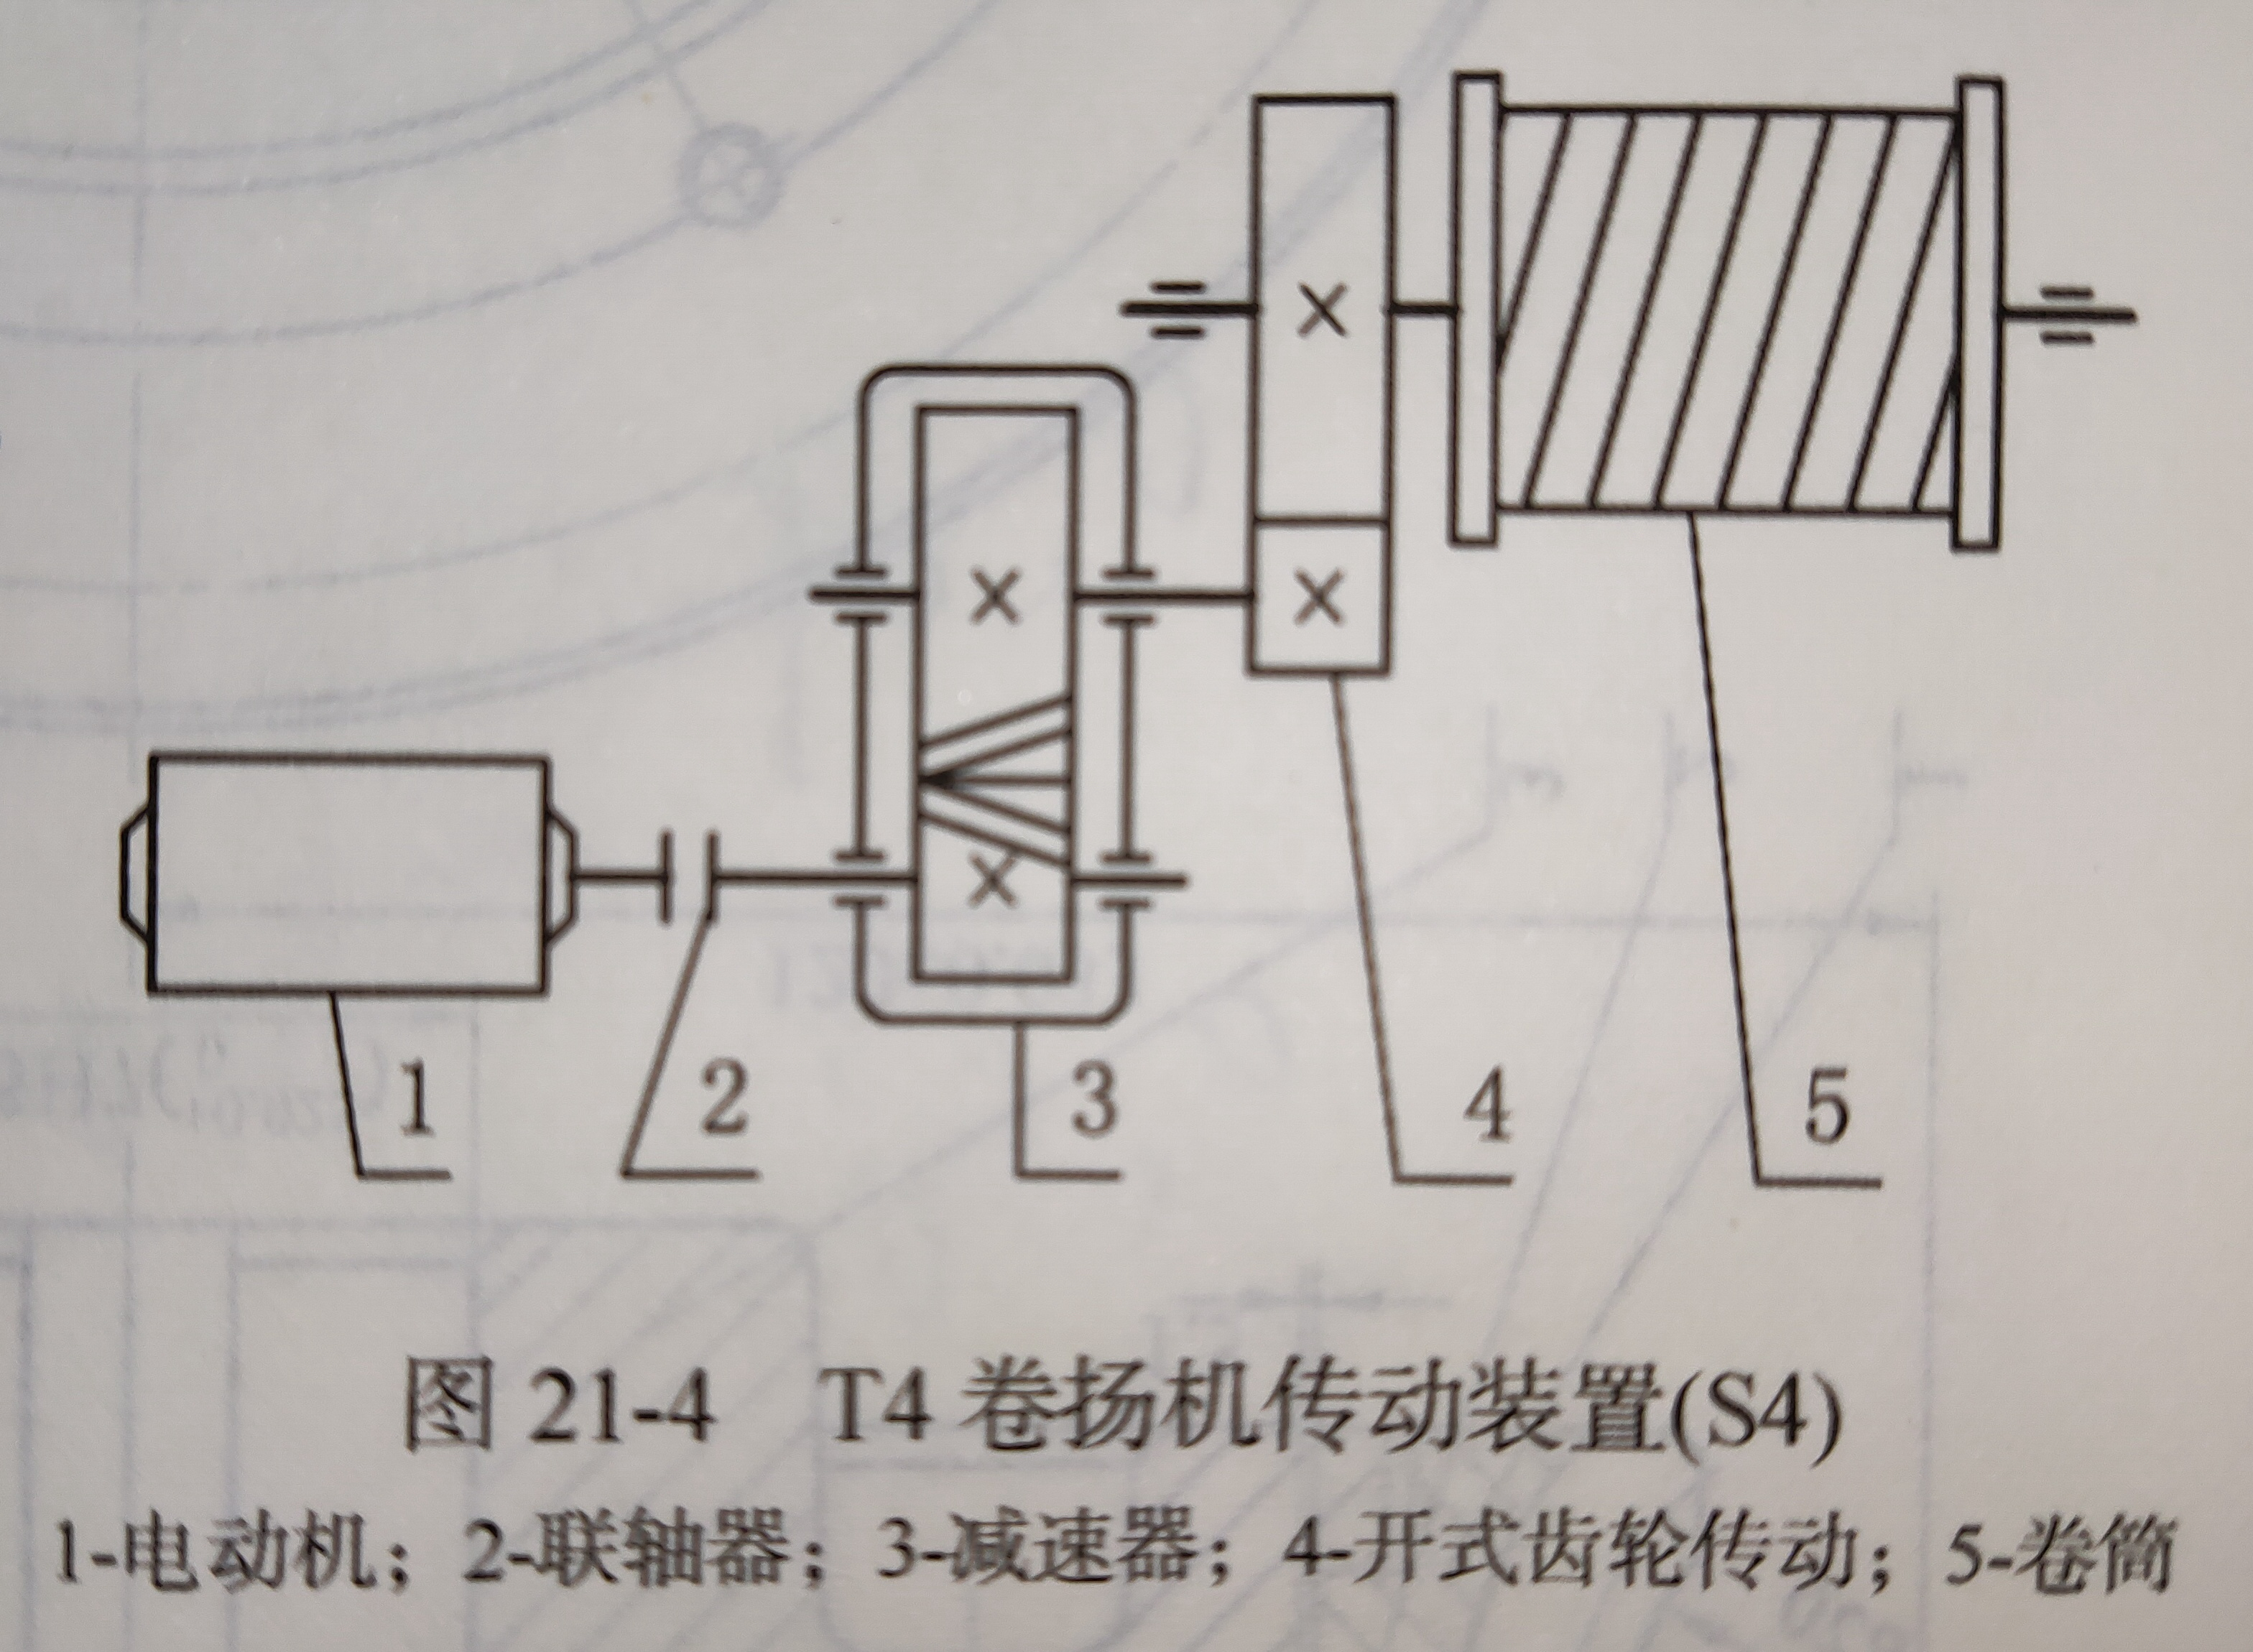
\includegraphics[scale=0.1]{graphic/1.jpg}
    \caption{卷扬机传动装置}
\end{figure}
% 这是引用测试 \cite{Barlow.2015}  暂时不进行参考文献的收录,等到最后去点main文件的参考文献的注释
\subsection{工作情况}
轻微振动载荷;单向传动;成批生产;长期使用,轴承寿命10000小时
\subsection{设计数据}
\begin{tabular}{|p{12em}|p{8em}|}
    \hline
    卷筒圆周力$F/N$     & 2500 \\
    \hline
    卷筒转速$n/(r/min)$ & 80   \\
    \hline
    卷筒直径$D/mm$      & 400  \\
    \hline
\end{tabular}
    \section{传动装置方案拟定}

传动方案说明

采用闭式斜齿圆柱齿轮传动,能适应在繁重及恶劣的条件下长期工作,且使用维护方便。斜齿轮传动的平稳性较直齿轮传动好,适合用在高速级或要求传动平稳的场合。由于开式齿轮传动的工作环境较差,润滑条件不好,磨损较为严重,寿命较短,布置在低速级。

由于斜齿轮在传动过程中会产生轴向力,其螺旋升角不宜过大。设计时一般取$\beta =8^\circ\sim 20^\circ$。
    \section{选择电动机}

\subsection{计算电动机所需功率}
输出功率
\begin{equation}
    P= \frac{T\omega}{9550}=\frac{2500 \times \frac{450}{2} \times 10^{-3} \times 80}{9550} = 9.42kw
\end{equation}

查表的各个传动装置的传动效率及其传动比

\begin{tabular}{|c|c|p{12em}|c|c|}
    \hline
    联轴器 & 球滚子轴承 & 斜齿圆柱齿轮(闭式传动,精度等级8级) & 圆柱齿轮(开式传动) & 运输滚筒 \\
    \hline
    0.99   & 0.99       & 0.97                                  & 0.96                 & 0.96     \\
    \hline
    1      & 1          & 3$\sim$6                              & 4$\sim$6             & 1        \\
    \hline
\end{tabular}

总传动效率为
\begin{equation}
    \eta = 0.99^4 \times 0.97 \times 0.96^2 = 0.859
\end{equation}

电动机所需额定功率

\begin{equation}
    P_d = \frac{P}{0.857} = 10.97
\end{equation}

\subsection{选择电动机}
查表得理论传动比范围是 12$\sim$36。可选择的电动机转速范围为:$n_d = i_a \times n = (12 \sim 36)\times 80=(960 \sim 2880)r/min$。总的电动机选择方案共有以下三种情况。

\begin{tabular}{|c|c|c|c|}
    \hline
    方案 & 电机型号      & 额定功率$kW$ & 同步转速$(r/min)$ \\
    \hline
    1    & $YE3-160M1-2$ & 11           & 2940              \\
    \hline
    2    & $YE3-160M-4$  & 11           & 1470              \\
    \hline
    3    & $YE3-160L-6$  & 11           & 975               \\
    \hline
\end{tabular}

考虑到低转速的电动机,转矩大,且传动装置的总传动比较小、体积小、重量较小。选定电动机型号为:$YE3-160L-6$,额定功率为$11kW$,同步转速为$975r/min$,重量为$140kg$.

\begin{figure}[h]
    \centering
    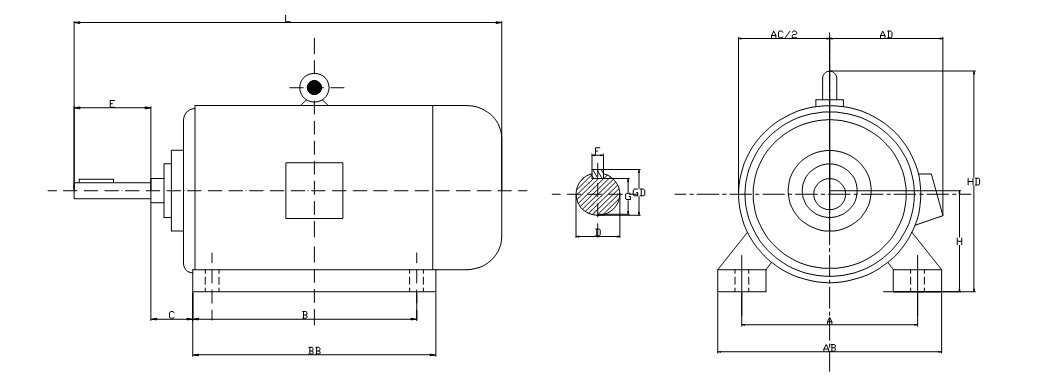
\includegraphics[scale=0.5]{graphic/3-1.png}
    \caption{电动机尺寸}
\end{figure}

\begin{tabular}{|c|p{8em}|c|c|c|c|}
    \hline
    中心高 & 外形尺寸                        & 底脚安装尺寸    & 地脚螺栓孔直径 & 轴伸尺寸        & 装键部位尺寸    \\
    \hline
    $H$    & $L\times (AC/2+AD)\times HD$    & $A\times B$     & $K$            & $D\times E$     & $F\times GD$    \\
    \hline
    160    & $760\times 380\times 425      $ & $254\times 253$ & $14.5      $   & $42\times 110 $ & $12\times 37  $ \\
    \hline
\end{tabular}

\subsection{分配各级传动比}
(1)总传动比的计算

由选定的电动机满载转速$n_m$和工作机主动轴的转速$n$,可得传动装置总传动比为
\begin{equation}
    i_a = \frac{n_m}{n} = \frac{975}{90} = 12.19
\end{equation}

(2)分配传动装置传动比

取高速级传动比为$i_a = 4.8 $, 则开式齿轮传动传动比为
\begin{equation}
    i_2 = \frac{i_a}{i_1}=2.5
\end{equation}

\subsection{计算各轴转速、功率和转矩}
\subsubsection{电动机输出参数}
\[
    P_0 = 10.97kW
\]
\[
    n_0 = n =975r/min
\]
\[
    T_0 = 9550\times \frac{P_0}{n_0}= \frac{10.97}{975} = 107.45N \cdot m
\]

\subsubsection{高速轴的参数}
\[
    P_1 = P_0 \times \eta_1 = 10.97 \times 1 =10.97 kW
\]
\[
    n_1 = n_0 =975 r/min
\]
\[
    T_1 = T_0 \times i_0 \times \eta_{01} = 107.45 N \cdot m
\]

\subsubsection{低速轴的参数}
\[
    P_2 = P_1 \times \eta_{2} \eta_{3} = 10.53 kW
\]
\[
    n_2 = \frac{n}{n_1} = 203.13 r/min
\]
\[
    T_2 = T_1 \times \eta_{2} \eta_{3} = 495.13 N \cdot m
\]
\subsubsection{工作机轴的参数}
\[
    P_3 = P_2 \times \eta_{2} \eta_{3} = 10.11 kW
\]
\[
    n_3 = \frac{n_2}{i_2} = 81.25r/min
\]
\[
    T_3 = T_2 \times \eta_{2} \eta_{3} = 1188.31N \cdot m \\
\]

各轴运动和动力参数的计算结果汇总于下表

\begin{tabular}{|c|c|c|c|c|}
    \hline
    轴名称              & 电机轴   & 高速轴   & 低速轴   & 工作机轴  \\
    \hline
    转速$n/(r/min)$     & $975$    & $ 975$   & $203.13$ & 81.25     \\
    \hline
    功率$P/kW$          & $10.97$  & $10.97$  & $10.53$  & $10.11$ \\
    \hline
    转矩$T/(N \cdot m)$ & $107.45$ & $107.45$ & $495.13$  & $1188.31$   \\
    \hline
\end{tabular}
    \section{齿轮零件的设计计算\cite{杨可桢}}

\subsection{高速级齿轮计算}
\begin{tabular}{p{32em}|p{5em}}
    \hline
    计算及说明&结果\\
    \hline
    高速级齿轮传动设计& \\
    $p=10.97kW,n=975r/min,T=1.07\times 10^5N\cdot mm,u=4.8$&\\
    1.选择齿轮材料、精确等级和确定需用应力 &\\
    (1)齿轮材料& \\

    小齿轮选用$20CrMnTi$,渗碳淬火,$HBS=59$&\\
    $[\sigma_H]=1500MPa,[\sigma_{FE}]=850MPa$&\\

    大齿轮选用$20Cr$,渗碳淬火,$HBS =59$&\\
    $[\sigma_H]=1500MPa,[\sigma_{FE}]=850MPa$&\\

    (2)选用7级精度 &\\
    
    2.选择齿轮的参数 & \\
    小齿轮的齿数$z_1=24$&$z_1=24$\\
    大齿轮的齿数$z_2=u\times z_1=115.2$&$Z_2=116$\\
    初选螺旋角$\beta = 15^\circ$&$\beta =15^\circ$\\
    一般可靠度$S_H= 1,S_F =1.25,Z_E = 189.8\sqrt[2]{MPa}$& \\
    齿宽系数$\phi_d=0.8$& \\

    3.按齿轮弯曲强度进行计算 &\\
    计算齿形系数$Z_{v}=\frac{z}{(cos \beta)^3}$ & $z_{v1}=21.08$\\
                         &$z_{v2}=128$\\

    查表得$Y_{Fa1}=2.88,Y_{Fa2}=2.22,Y_{Sa1}=1.57,Y_{Sa2}=1.80$&\\
    计算$\mu =\frac{Y_{Fa}{Y_Sa}}{[\sigma_F]}$& $\mu_1=0.0095$,$\mu_2=0.0084$\\

    进行弯曲强度计算& \\
    法向模数 $m_n\geq\sqrt[3]{\frac{2KT}{\phi_d z_1^2}\cdot\frac{Y_{Fa}Y_{Sa}}{[\sigma_{F1}]}\cdot(cos \beta)^2}$&\\

    $=\sqrt[3]{\frac{2\times 1.1\times 1.07\times 10^5}{0.8\times 24^2}\times 0.0095 \times (cos 15^\circ)^2}=1.67$& $m_n = 2mm$\\

    中心距$a=\frac{m_n\times (z_1+ z_2)}{2(cos \beta)}=\frac{2\times (24+116)}{2\times (cos15^\circ)}$&$a=145mm$\\

    螺旋角 $\beta =arccos(\frac{m_n(z_1+ z_2)}{2a})=arccos(\frac{2\times (19+92)}{2\times 115})=15^\circ 9'21''$&$\beta =15^\circ 9'21''$\\

    分度圆直径$d=\frac{m_n z}{cos \beta}$&$d_1=49.73mm$,$d_2=240.4mm$\\

    齿宽 $b=\phi_d d_1=0.8\times 49.73=39.78mm$&\\
    圆整取$b_1=45mm,b_2=40mm$&\\
    齿顶圆直径$d_1=53.7mm,d_2=244.4mm$

    4.验算齿面接触强度&\\
    将参数带入得&\\
    $\sigma_H =3.54Z_E Z_\beta\sqrt{\frac{KT}{bd_1^2}\frac{u+1}{u}}$& $\sigma_{H1}=790MPa<[\sigma_{H1}]$\\
    \hline
\end{tabular}
\newpage
\begin{tabular}{p{32em}|p{5em}}
    \hline
    & $\sigma_{H2}=455MPa<[\sigma_{H2}]$\\
    5.齿轮圆周速度$v=\frac{\pi d_1 n_1 }{60 \times 1000}=\frac{\pi\times 49.73\times 975}{60000}m/s =2.54m/s$& $v = 2.54m/s$\\
    \hline
\end{tabular}

\subsection{低速级齿轮计算}
\begin{tabular}{p{32em}|p{5em}}
    \hline
    计算及说明 & 结果\\
    \hline
    低速级齿轮传动设计 & \\
    $p = 10.53kW, n= 203.15r/min,T=4.95\times 10^5 N\cdot mm,u = 2.5$ & \\
    1.选择齿轮材料、精度等级和确定许用应力 & \\
    (1)齿轮材料 & \\

    小齿轮选用$40Cr$,表面淬火,$HRC = 48\sim 55$ & \\
    $\sigma_H=1180MPa,\sigma_{FE}=720MPa$& \\
    大齿轮选用$45$钢,表面淬火,$HRC =40\sim 50$ & \\
    $\sigma_H=1135MPa,\sigma_{FE}=690MPa$& \\

    (2)选用7级精度 & \\

    2.选择齿轮的参数 & \\
    小齿轮的齿数$z_1=19$ &$z_1 =19$ \\
    大齿轮的齿数$z_2=i\times z_1=47.5$,取$z_2=48$ & $z_2=48$\\

    3.按齿根弯曲疲劳强度设计 & \\
    (1)由一般可靠度,齿轮双向传动,选择$S_H = 1,S_F = 1.25,K=1.1$,齿宽系数$\phi_d=0.4$& \\
    
    计算$[\sigma_{F}]=\frac{0.7\sigma_{FE}}{S_F}$ & $[\sigma_{F1}]=403.2MPa$\\ 
                    &$[\sigma_{F2}]=386.4MPa$\\

    $[\sigma_{H}]=\frac{\sigma_{H}}{S_H}$ & $[\sigma_{H1}]=1180MPa$\\ 
                    &$[\sigma_{H2}]=1135MPa$\\

    查表得$Y_{Fa1}=2.98,Y_{Fa2}=2.38,Y_{Sa1}=1.55,Y_{Sa2}=1.69$ & \\

    分别计算$\frac{Y_{Fa}\cdot {Y_Sa}}{[\sigma_H]}$ & 分别得到$0.0115,0.0104$\\

    计算$m \geq \sqrt[3]{\frac{2KT}{\phi_d z_1^2}\cdot \frac{Y_{Fa}Y_{Sa}}{[\sigma F]}}$ & $m\geq4.43$,取$m=5$\\

    中心距$a = \frac{m(z_1 + z_2)}{2} $ & $a= 134mm$\\

    分度圆直径$d=zm$ &$d_1= 95mm$,$d_2=240$\\

    齿宽$b=\phi d=38$&$b_1=45mm$,$b_2=40mm$\\
    \hline
\end{tabular}

\subsection{高速级齿轮参数总结}
\begin{tabular}{|c|c|c|}
    \hline
        & 小齿轮&大齿轮\\
    \hline
    模数$m$ & $2mm$ & $2mm$\\
    \hline
    齿数$z$&$24$&$116$\\
    \hline
    螺旋角$\beta$&右旋$15^\circ 9'21''$&左旋$15^\circ 9'21''$\\
    \hline
    齿宽$b$&$45mm$&$40mm$\\
    \hline
    分度圆直径$d$&$49.73mm$&$190.63mm$\\
    \hline
    齿顶高系数$h_a$&$1.0$&$1.0$\\
    \hline
    顶隙系数$c$&$0.25$&$0.25$\\
    \hline
    齿顶高$h_a$&$2mm$&$2mm$\\
    \hline
    齿根高$h_f$&$2.5mm$&$2.5mm$\\
    \hline
    全尺高$h$&$4.5mm$&$4.5mm$\\
    \hline
\end{tabular}

\subsection{低速级齿轮参数总结}
\begin{tabular}{|c|c|c|}
    \hline
        & 小齿轮&大齿轮\\
    \hline
    模数$m$ & $5mm$ & $5mm$\\
    \hline
    齿数$z$&$19$&$48$\\
    \hline
    齿宽$b$&$45mm$&$40mm$\\
    \hline
    分度圆直径$d$&$95mm$&$240mm$\\
    \hline
    齿顶高系数$h_a$&$1.0$&$1.0$\\
    \hline
    顶隙系数$c$&$0.25$&$0.25$\\
    \hline
    齿顶高$h_a$&$5mm$&$5mm$\\
    \hline
    齿根高$h_f$&$6.25mm$&$6.25mm$\\
    \hline
    全尺高$h$&$11.25mm$&$11.25mm$\\
    \hline
\end{tabular}
    \section{轴的计算与校核}
\subsection{高速轴设计计算}
\subsubsection{计算得到的相关运动参数}
    \[
        转速 n = 975r/min;功率 P =10.97kW;轴的转矩T=1.07\times 10^5 N\cdot mm
    \]
\subsubsection{轴的材料选择确定许用应力}
    选择$40Cr$调质,硬度为$280HBS$,许用弯曲应力为$[\sigma]=60MPa$
\subsubsection{按扭转强度概略计算轴的最小直径}
    材料的$C:107\sim 98$
    \[
        d \geq C\times \sqrt[3]{\frac{P}{n}}=(107\sim 98)\times \sqrt[3]{\frac{10.97}{975}}=(23.98\sim 21.96)mm
        \]

    最小轴端界面开一个键槽,将轴径增大$7\%$,得出轴的最小直径$(26.429\sim 23.5)mm$,查的标准轴的直径$d=32mm$。
\begin{figure}[h]
    \centering
    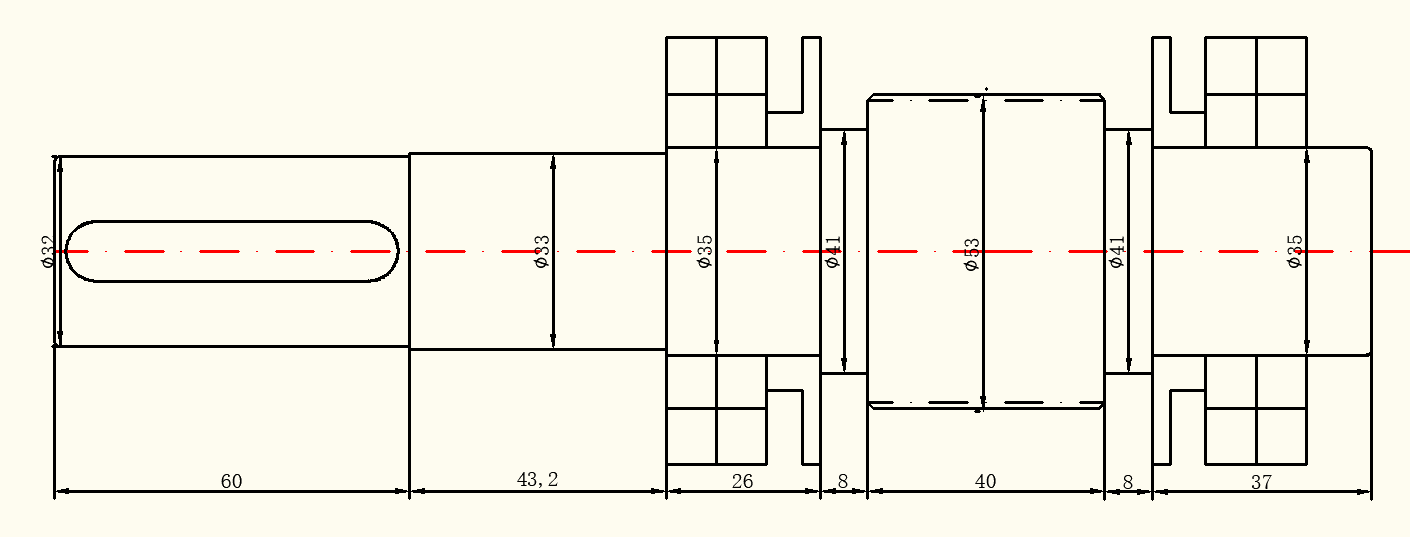
\includegraphics[scale=0.5]{graphic/5-1.png}
    \caption{轴的结构设计图}
\end{figure}

(1)高速轴与联轴器配合

标准轴径为$d_{12}=32mm$,$l_{12}$略大于联轴器轴孔长度$L=60mm$,取$l_{12}=64mm$。

选择弹性套柱销联轴器$LT6$,公称转矩$355N\cdot mm$,许用转速$3800r/min$。

选用普通平键,A型键,$b\times h=10\times 8$,取键长$L=56mm$。

(2)初步选择滚动轴承

因承受径向载荷的作用,选用角接触球轴承,选择型号$7207AC$ ,尺寸为$b\times D \times B=35\times 72 \times 17$,定位肩高度$41mm$。

轴承采用挡油环进行轴向固定。取$d_{45}=d_{46}=41mm$。

(3)由于齿轮的直径较小,为了保证齿轮轮体的强度,将齿轮和轴做为齿轮轴。因此上$l_{56}=45mm,d{56}=54mm$

(4)使用凸缘式轴承盖,轴承盖厚度$e=dn=1.2\times 6mm$,垫片厚度$\delta t=2mm$,使轴承盖便于拆卸,保证轴承盖外端面与联轴器有一定距离$K=24$,因此$L_{23}=43.2mm$,

(5)保证旋转零件端面至箱体内壁的距离$a=10\sim 15mm$,现取$L_{78}=37mm$。

确定的轴的尺寸见下表

\begin{tabular}{|c|c|c|c|c|c|c|c|}
    \hline
    直径& $32$&$33$&$35$&$41$&$53$&$41$&$35$\\
    \hline
    长度&$60$&$43.2$&$26$&$8$&$40$&$8$&$37$\\
    \hline
\end{tabular}

\subsubsection{受力分析与校核}
\begin{figure}[h]
    \centering
    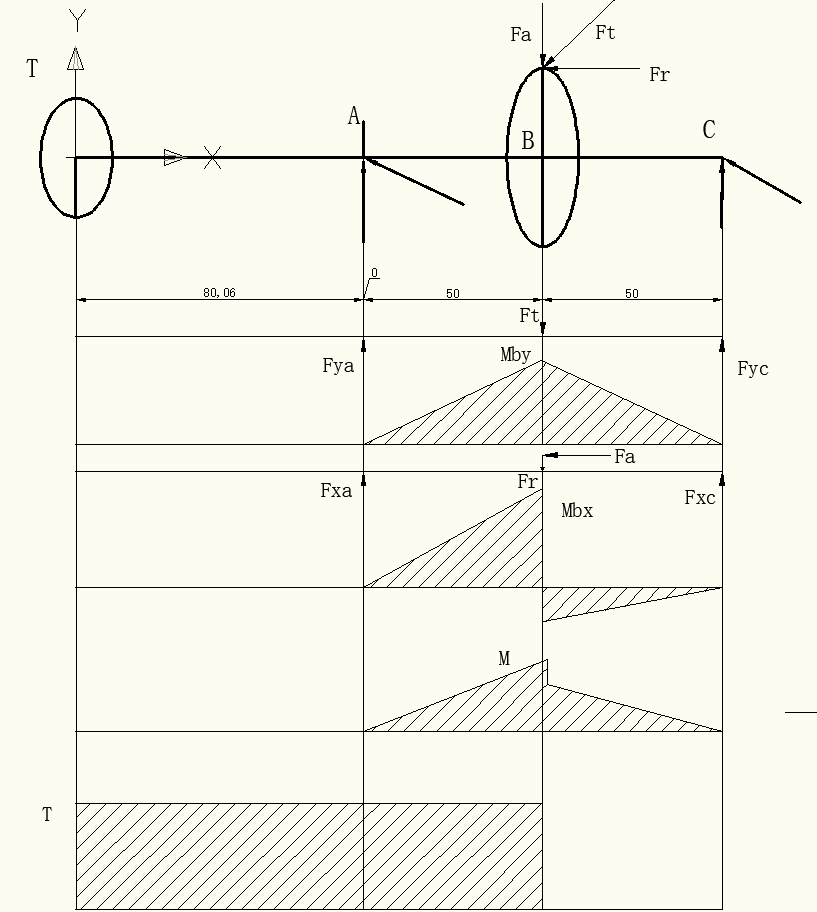
\includegraphics[scale=0.7]{graphic/5-2.png}
    \caption{高速轴的受力分析简图}
    \label{img1}
\end{figure}

(1)小齿轮受力情况如下:
\begin{align}
    \text{圆周力}       \qquad   F_{t1}=2\times \frac{T}{d_1}=4323.94N \\
    \text{径向力} \qquad          F_{r1}=F_{t1}\frac{tan\alpha_n}{cos \beta}=1630.50N\\
    \text{轴向力}       \qquad          F_{a1}=F_{t1}\times tan\beta =1171.23\\
    \text{电动机转矩} \qquad\qquad      T=107.45N\cdot m
\end{align}

齿宽中点距左支点距离 $L_2 =50mm$

齿宽中点距右支点距离 $L_3 =50mm$

(2)计算轴的支反力

垂直面支反力
\begin{align*}
    F_{ya}=\frac{F_{t1}L_3}{L_2+L_3}=2161.97N\\
    F_{yc}=\frac{F_{t1}L_2}{L_2+L_3}=2161.97N
\end{align*}

水平面支反力
\begin{align*}
    F_{xa}=\frac{F_{a1}{\frac{d_1}{2}}+F_{r1}L_3}{L_2+L_3} =1106.47N \\
    F_{xc}=\frac{F_{r1}{L_2}-F_{a1}\frac{d_1}{2}}{L_2+L_3}=524.2N
\end{align*}

(3)计算轴的弯矩,绘制弯矩图如\ref{img1}

截面$B$处的垂直弯矩
\[
    M_{by}=F_{ya}L_2=108098.5N\cdot mm
\]
截面$B$处的水平弯矩
\[
    M_{bx1}=F_{xa}L_2=55337N\cdot mm
\]
\[
    M_{bx2}=F_{xc}L_3=-26210N\cdot mm
\]
截面处的合成弯矩
\begin{align*}
    M_1=\sqrt{M_{by}^2+M_{bx1}^2}=121439.16N\cdot mm\\
    M_2=\sqrt{M_{by}^2+M_{bx2}^2}=111230.62N\cdot mm
\end{align*}

(4)画出电机施加的转矩图

(5)校核轴上承受最大弯矩和转矩的截面,即截面$B$

材料的抗弯截面系数
\[
    W=\frac{\pi d_1^2}{32}=12052mm^3
\]
弯曲应力
\[
    \sigma = \frac{M_1}{W} =10.76MPa
\]
抗扭截面系数
\[
    W_T=\frac{\pi d_1^2}{16}=24105mm^3
\]
切应力
\[
    \tau = \frac{T}{W}_T =4.46MPa
\]
按转矩脉动变化$\alpha =0.6$
\[
    \sigma_e =\sqrt{\sigma^2+4\times (\alpha \times \tau)^2}=11.65MPa
\]
材料选用$40Cr$调质,抗拉极限强度$\sigma_B=734MPa$,轴的许用弯曲应力$[\sigma_{-1b}=60MPa]$,因此设计的轴有足够的强度。   



\subsection{低速轴设计计算}
\subsubsection{计算得到的相关运动参数}
\[
        转速 n = 203.15r/min;功率 P =10.53kW;轴的转矩T=4.95\times 10^5 N\cdot mm
\]
\subsubsection{轴的材料选择确定的许用应力}
    选择$45$钢调质,硬度为$280HBS$,许用弯曲应力为$[\sigma]=60MPa$
\subsubsection{按扭转强度概略计算轴的最小直径}
材料的$C:118\sim 107$
    \[
        d \geq C\times \sqrt[3]{\frac{P}{n}}=(118\sim 107)\times \sqrt[3]{\frac{10.53}{203.15}}=(44\sim 40)mm
    \]
    最小轴端界面开一个键槽,将轴径增大$7\%$,得出轴的最小直径$(47.08\sim 42.8)mm$,查的标准轴的直径$d=50mm$。
\begin{figure}[h]
    \centering
    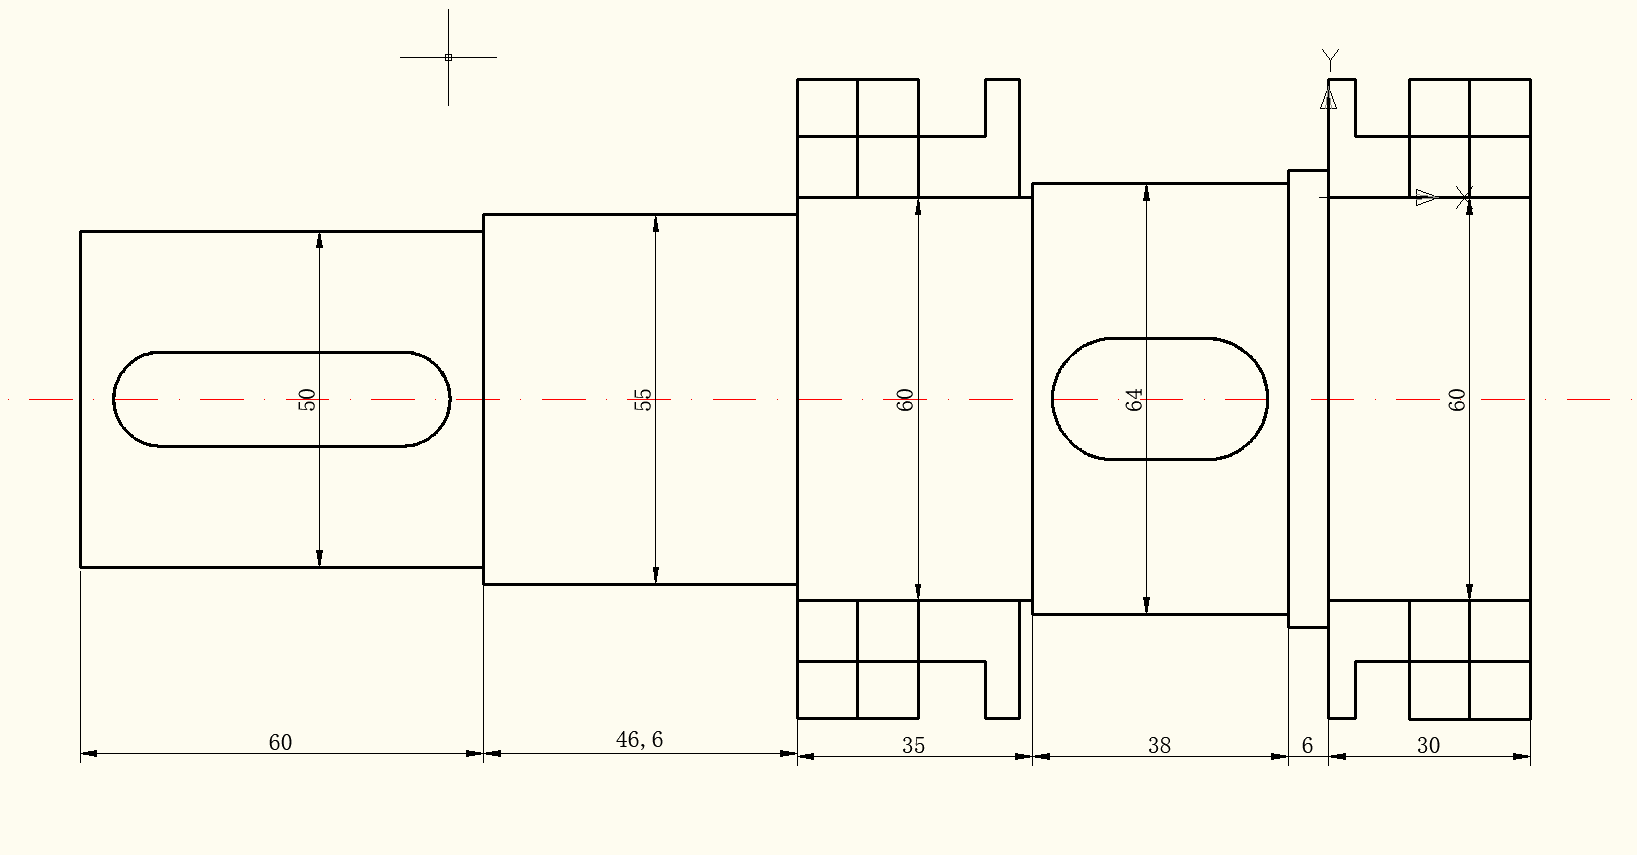
\includegraphics[scale=0.4]{graphic/5-3.png}
    \caption{轴的结构设计图}
\end{figure}

(1)低速轴与外齿轮配合

标准轴径为$d_{12}=50mm$,$l_{12}$略大于齿轮齿宽$L=40mm$,取$l_{12}=60mm$。

选用普通平键,$A$型键,$b\times h=14\times 9$,取键长$L=40mm$。

(2)初步选择滚动轴承

因承受径向载荷的作用,选用角接触球轴承,选择型号$7012AC$ ,尺寸为$b\times D \times B=60\times 95 \times 18$,定位肩高度$68mm$。

轴承采用挡油环进行轴向固定。取$d_{56}=68mm$。

(3)取安装齿轮处的轴段的直径$d_{45} = 64mm$;齿轮的左端与左轴承之间采用套筒定位。已知大齿轮轮毂的宽度为$b=40 mm$,为了使套筒端面可靠地压紧齿轮,此轴段应略短于轮毂宽度,故取$l_{45} = 38 mm$。

(4)使用凸缘式轴承盖,轴承盖厚度$e=dn=1.2\times 8mm$,垫片厚度$\Delta t=2mm$,使轴承盖便于拆卸,保证轴承盖外端面与联轴器有一定距离$K=24$,因此$L_{23}=46.6mm$。

(5)保证旋转零件端面至箱体内壁的距离$a=10\sim 15mm$,现取$L_{78}=30mm$。

确定的轴的尺寸见下表

\begin{tabular}{|c|c|c|c|c|c|c|}
    \hline
    直径& $50$&$55$&$60$&$64$&$68$&$60$\\
    \hline
    长度&$60$&$46.6$&$35$&$38$&$6$&$30$\\
    \hline
\end{tabular}
\subsubsection{受力分析与校核}
(1)小齿轮受力情况如下:
\begin{align}
    \text{圆周力}       \qquad   F_{t2}=2\times \frac{T}{d_2}=4119.22N \\
    \text{径向力} \qquad          F_{r2}=F_{t2}\frac{tan\alpha_n}{cos \beta}=1553.3N\\
    \text{轴向力}       \qquad          F_{a2}=F_{t2}\times tan\beta =1115.77\\
    \text{电动机转矩} \qquad\qquad      T=495.13N\cdot m
\end{align}

齿宽中点距左支点距离 $L_2 =42mm$

齿宽中点距右支点距离 $L_3 =46mm$

\begin{figure}[h]
    \centering
    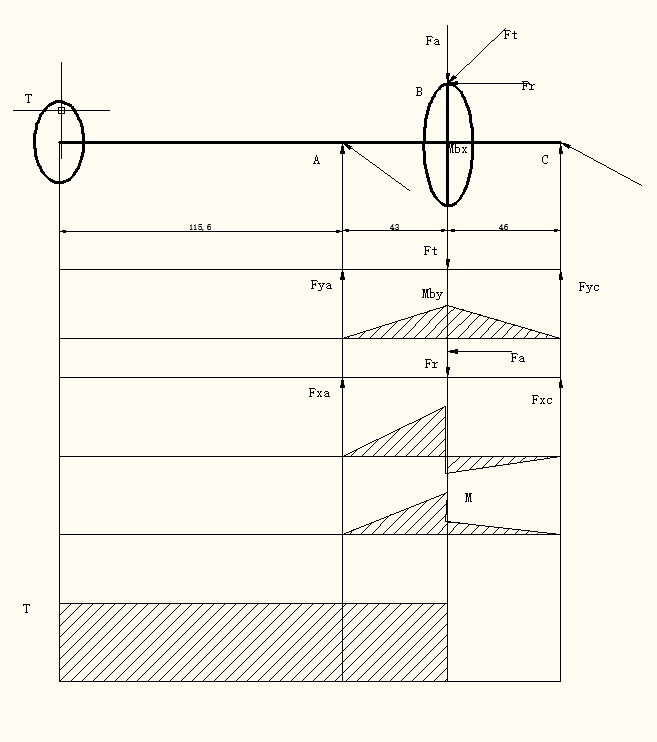
\includegraphics[scale=0.8]{graphic/5-4.png}
    \caption{高速轴的受力分析简图}
    \label{img2}
\end{figure}

(2)计算轴的支反力

垂直面支反力
\begin{align*}
    F_{ya}=\frac{F_{t2}L_3}{L_2+L_3}=2129.04N\\
    F_{yc}=\frac{F_{t2}L_2}{L_2+L_3}=1990.18N
\end{align*}

水平面支反力
\begin{align*}
    F_{xa}=\frac{F_{a2}{\frac{d_2}{2}}+F_{r2}L_3}{L_2+L_3} =1997.77N \\
    F_{xc}=\frac{F_{r2}{L_2}-F_{a2}\frac{d_2}{2}}{L_2+L_3}=-444.47N
\end{align*}

(3)计算轴的弯矩,绘制弯矩图如\ref{img2}

截面$B$处的垂直弯矩
\[
    M_{by1}=F_{ya}L_2=91548.72N\cdot mm
\]
\[
    M_{by2}=F_{ya}L_3=91548.28N\cdot mm
\]
截面$B$处的水平弯矩
\[
    M_{bx1}=F_{xa}L_2=85904.11N\cdot mm
\]
\[
    M_{bx2}=F_{xc}L_3=20445.62N\cdot mm
\]
截面处的合成弯矩
\begin{align*}
    M_1=\sqrt{M_{by1}^2+M_{bx1}^2}=125541.56N\cdot mm\\
    M_2=\sqrt{M_{by2}^2+M_{bx2}^2}=93803.58N\cdot mm
\end{align*}

(4)画出电机施加的转矩图

(5)校核轴上承受最大弯矩和转矩的截面,即截面$B$

材料的抗弯截面系数
\[
    W=\frac{\pi d_1^2}{32}=25735.93mm^3
\]
弯曲应力
\[
    \sigma = \frac{M_1}{W} =4.88MPa
\]
抗扭截面系数
\[
    W_T=\frac{\pi d_1^2}{16}=51471.85mm^3
\]
切应力
\[
    \tau = \frac{T}{W}_T =9.61MPa
\]
按转矩脉动变化$\alpha =0.6$
\[
    \sigma_e =\sqrt{\sigma^2+4\times (\alpha \times \tau)^2}=12.52MPa
\]
材料选用$45$钢调质,抗拉极限强度$\sigma_B=600MPa$,轴的许用弯曲应力$[\sigma_{-1b}=60MPa]$,因此设计的轴有足够的强度。   

    \section{键连接的选择和计算}
\subsection{高速轴与联轴器连接校核}
选用$A$型键,查表得$b\times h=10mm\times 8mm(GB/T 1096-2003)$,键长$56mm$。
键得工作长度为$l=L-b=46mm$。

工作面的挤压应力
\[
    \sigma_p = \frac{4\times T}{h\times l\times d}=95MPa
\]

材料为钢,许用挤压应力为$[\sigma_p]=100\sim 120MPa$,满足强度要求。
\subsection{低速轴与大齿轮连接校核}
选用$A$型键,查表得$b\times h=18mm\times 11mm(GB/T 1096-2003)$,键长$32mm$。
键得工作长度为$l=L-b=14mm$。

工作面的挤压应力
\[
    \sigma_p = \frac{4\times T}{h\times l\times d}=71MPa
\]
    
材料为钢,许用挤压应力为$[\sigma_p]=100\sim 120MPa$,满足强度要求。

\subsection{低速轴与开式齿轮连接校核}
选用$A$型键,查表得$b\times h=14mm\times 9mm(GB/T 1096-2003)$,键长$40mm$。
键得工作长度为$l=L-b=26mm$。

工作面的挤压应力
\[
    \sigma_p = \frac{4\times T}{h\times l\times d}=108MPa
\]
    
材料为钢,许用挤压应力为$[\sigma_p]=100\sim 120MPa$,满足强度要求。
    \section{滚动轴承的选择和计算}
\subsection{高速轴轴承的计算与校核}
(1)选用角接触球轴承,型号$7207AC$,尺寸$d\times D\times B=35\times 72\times 17$,基本额定动载荷$Cr=30.5kN$。轴承采用正装方式。

(2)轴承存在轴向载荷$F_a=1171.23N$,合成支撑反力$F_1=2162.47N,F_2=2224.6N$。
由轴承的内部轴向力公式
\[
    F_s=eF
\]
对角接触球轴承$e=0.68$。计算得到$F_{s1}=0.68\times 2162.47=1470.5N,F_{s2}=1512.73N$,考虑到轴向力的方向可以朝两个方向,假定轴向力从$F_1$指向$F_2$。
因此上得到
\[
    F_a+F_{s1}>F_{s2}
\]
此情况下,2端压紧$F_{a2}=F_a+F_{s1}=2641.7N$,1端放松$F_{a1}=F_{s1}=1470.5N$。
计算轴承的当量动载荷
\[
    \frac{F_{a1}}{F_1}=0.68
\]
\[
    \frac{F_{a2}}{F_2}=1.18
\]
查表得径向动载荷系数$X$和轴向动载荷系数分别为$Y$:
$X_1=1,Y_1=0;X_2=0.41,Y_2=0.87$
\begin{align}
    P_1=X_1 F_1+Y_1 F_{a1}=2162.46N\\
    P_2=X_2 F_2+Y_2 F_{a2}=3210.3N
\end{align}

齿轮受轻微冲击选择$f_P=1.1$,齿轮额定寿命$L_h=10000h$。
带入公式
\begin{equation}
    C_{r2}=\frac{f_P P_1}{f_1}(\frac{60n}{10^6} L_h)^{\frac{1}{3}}=29.53kN<[Cr]
\end{equation}
当其轴向力反向时计算得到
\[
    C_{r2}=22.02kN<[c_r]
\]
所以轴承预期寿命足够。

\subsection{低速轴轴承的计算与校核}
(1)选用角接触球轴承,型号$7012AC$,尺寸$d\times D\times B=60\times 95\times 18$,基本额定动载荷$Cr=36.2kN$。轴承采用正装方式。

(2)轴承存在轴向载荷$F_a=1115.77N$,合成支撑反力$F_1=4146.16N,F_2=1192.17N$。
由轴承的内部轴向力公式
\[
    F_s=eF
\]
对角接触球轴承$e=0.68$。计算得到$F_{s1}=0.68\times 4146.16=2819.39N,F_{s2}=810.67N$,考虑到轴向力的方向可以朝两个方向,假定轴向力从$F_1$指向$F_2$。
因此上得到
\[
    F_a+F_{s1}>F_{s2}
\]
此情况下,2端压紧$F_{a2}=F_a+F_{s1}=3935.16N$,1端放松$F_{a1}=F_{s1}=2819.39N$。
计算轴承的当量动载荷
\[
    \frac{F_{a1}}{F_1}=0.68
\]
\[
    \frac{F_{a2}}{F_2}=3.3
\]
查表得径向动载荷系数$X$和轴向动载荷系数分别为$Y$:
$X_1=1,Y_1=0;X_2=0.41,Y_2=0.87$
\begin{align}
    P_1=X_1 F_1+Y_1 F_{a1}=4146.16N\\
    P_2=X_2 F_2+Y_2 F_{a2}=3912.38N
\end{align}

齿轮受轻微冲击选择$f_P=1.1$,齿轮额定寿命$L_h=10000h$。
带入公式
\begin{equation}
    C_{r2}=\frac{f_P P_1}{f_1}(\frac{60n}{10^6} L_h)^{\frac{1}{3}}=22.61kN<[Cr]
\end{equation}
当其轴向力反向时计算得到
\[
    C_{r2}=22.61kN<[c_r]
\]
所以轴承预期寿命足够。
    \section{联轴器的选择}
(1)计算载荷

由表查得载荷系数$K=1.3$,计算转矩
\begin{equation}
    T_c = K\times T=1.3\times 107N\cdot m = 139.69N\cdot m
\end{equation}

(2)选择联轴器的型号

轴伸出端安装的联轴器初选型号为$LT6$弹性套柱销联轴器$(GB/T~4323-2017)$,公称转矩$T_n = 355N\cdot m$,许用转速$[n]=3800r/min$,Y型轴孔,主动端孔直径$d=42mm$,轴孔长度$L=112mm$。从动端孔直径$d=32mm$,轴孔长度$L=60mm$。
    \section{润滑与密封的选择,润滑剂牌号}
\subsection{轴承的润滑}
计算出高速轴和低速轴的速度因数$dn$分别等于$34125$和$12189$,其$dn<(2\sim 3)\times10^5mm\cdot r/min$,此时滚动轴承采用润滑脂润滑。

因此选用通用锂基润滑脂$(GB/T7324-2010)$,代号为$1$号,它适用于较宽温度范围的机械设备的润滑。

同时为了避免油脂被稀释,轴承与箱体内壁保持一定的距离且用挡油环将轴承与箱体隔开。
\subsection{齿轮的润滑}
计算出高速轴的齿轮转动速度
\[
    v= \pi dn=975r/min\times \pi \times 50\times 10^{-3} =5.1m/s
\]
低速轴的齿轮转动速度
\[
    v= \pi dn=203.15r/min\times \pi \times 240.4\times 10^{-3}=2.5m/s
\]
采用浸油润滑。浸油深度为0.7个齿高,同时不小于$10mm$。为了避免齿轮转动时将沉积在油池底部的污物搅起造成齿面磨损,大齿轮顶部距离箱体底面的距离$30mm$。大齿轮全尺高$h=2.23m_n=4.5mm$,取浸油深度为$10mm$,则油的深度为$40mm$。

根据齿轮圆周速度选用工业闭式齿轮油$(GB/T5903-2011)$,代号为$L-CKC320$。
\subsection{减速器的密封}
为防止箱体内润滑剂外泄和外部杂质进入箱体内部影响箱体工作,在构成箱体的各零件间,如箱盖与箱座间、外伸轴的输入、输出轴与轴承盖间,需设置不同形式的密封装置。对于无相对运动的接合面,常用密封胶、耐油橡胶垫圈等;对于旋转零件如外伸轴的密封,则需要根据其不同运动速度和密封要求考虑不同的密封件和结构。本设计中由于密封界面的相对速度较小,故采用接触式密封。输入轴与轴承盖间、输出轴与轴承盖间速度皆小于$3m/s$,故均采用半粗羊毛毡密封油圈。
    \section{其他技术说明}
\subsection{检查孔和检查孔盖}
检查传动零件的啮合情况,向箱体中注入润滑油。检查孔应设在上箱盖顶部能够直接观察到齿轮啮合部位的地方。检查孔为长方形,其大小应允许将手伸入箱内,以便检验齿轮啮合条件。检查孔盖用铸铁、钢板或有机玻璃制成,与箱体之间应加密封垫片。检查孔的盖板用螺钉固定在箱盖上。

检查孔和检查孔盖的主要尺寸设计如下:
\begin{figure}[h]
    \centering
    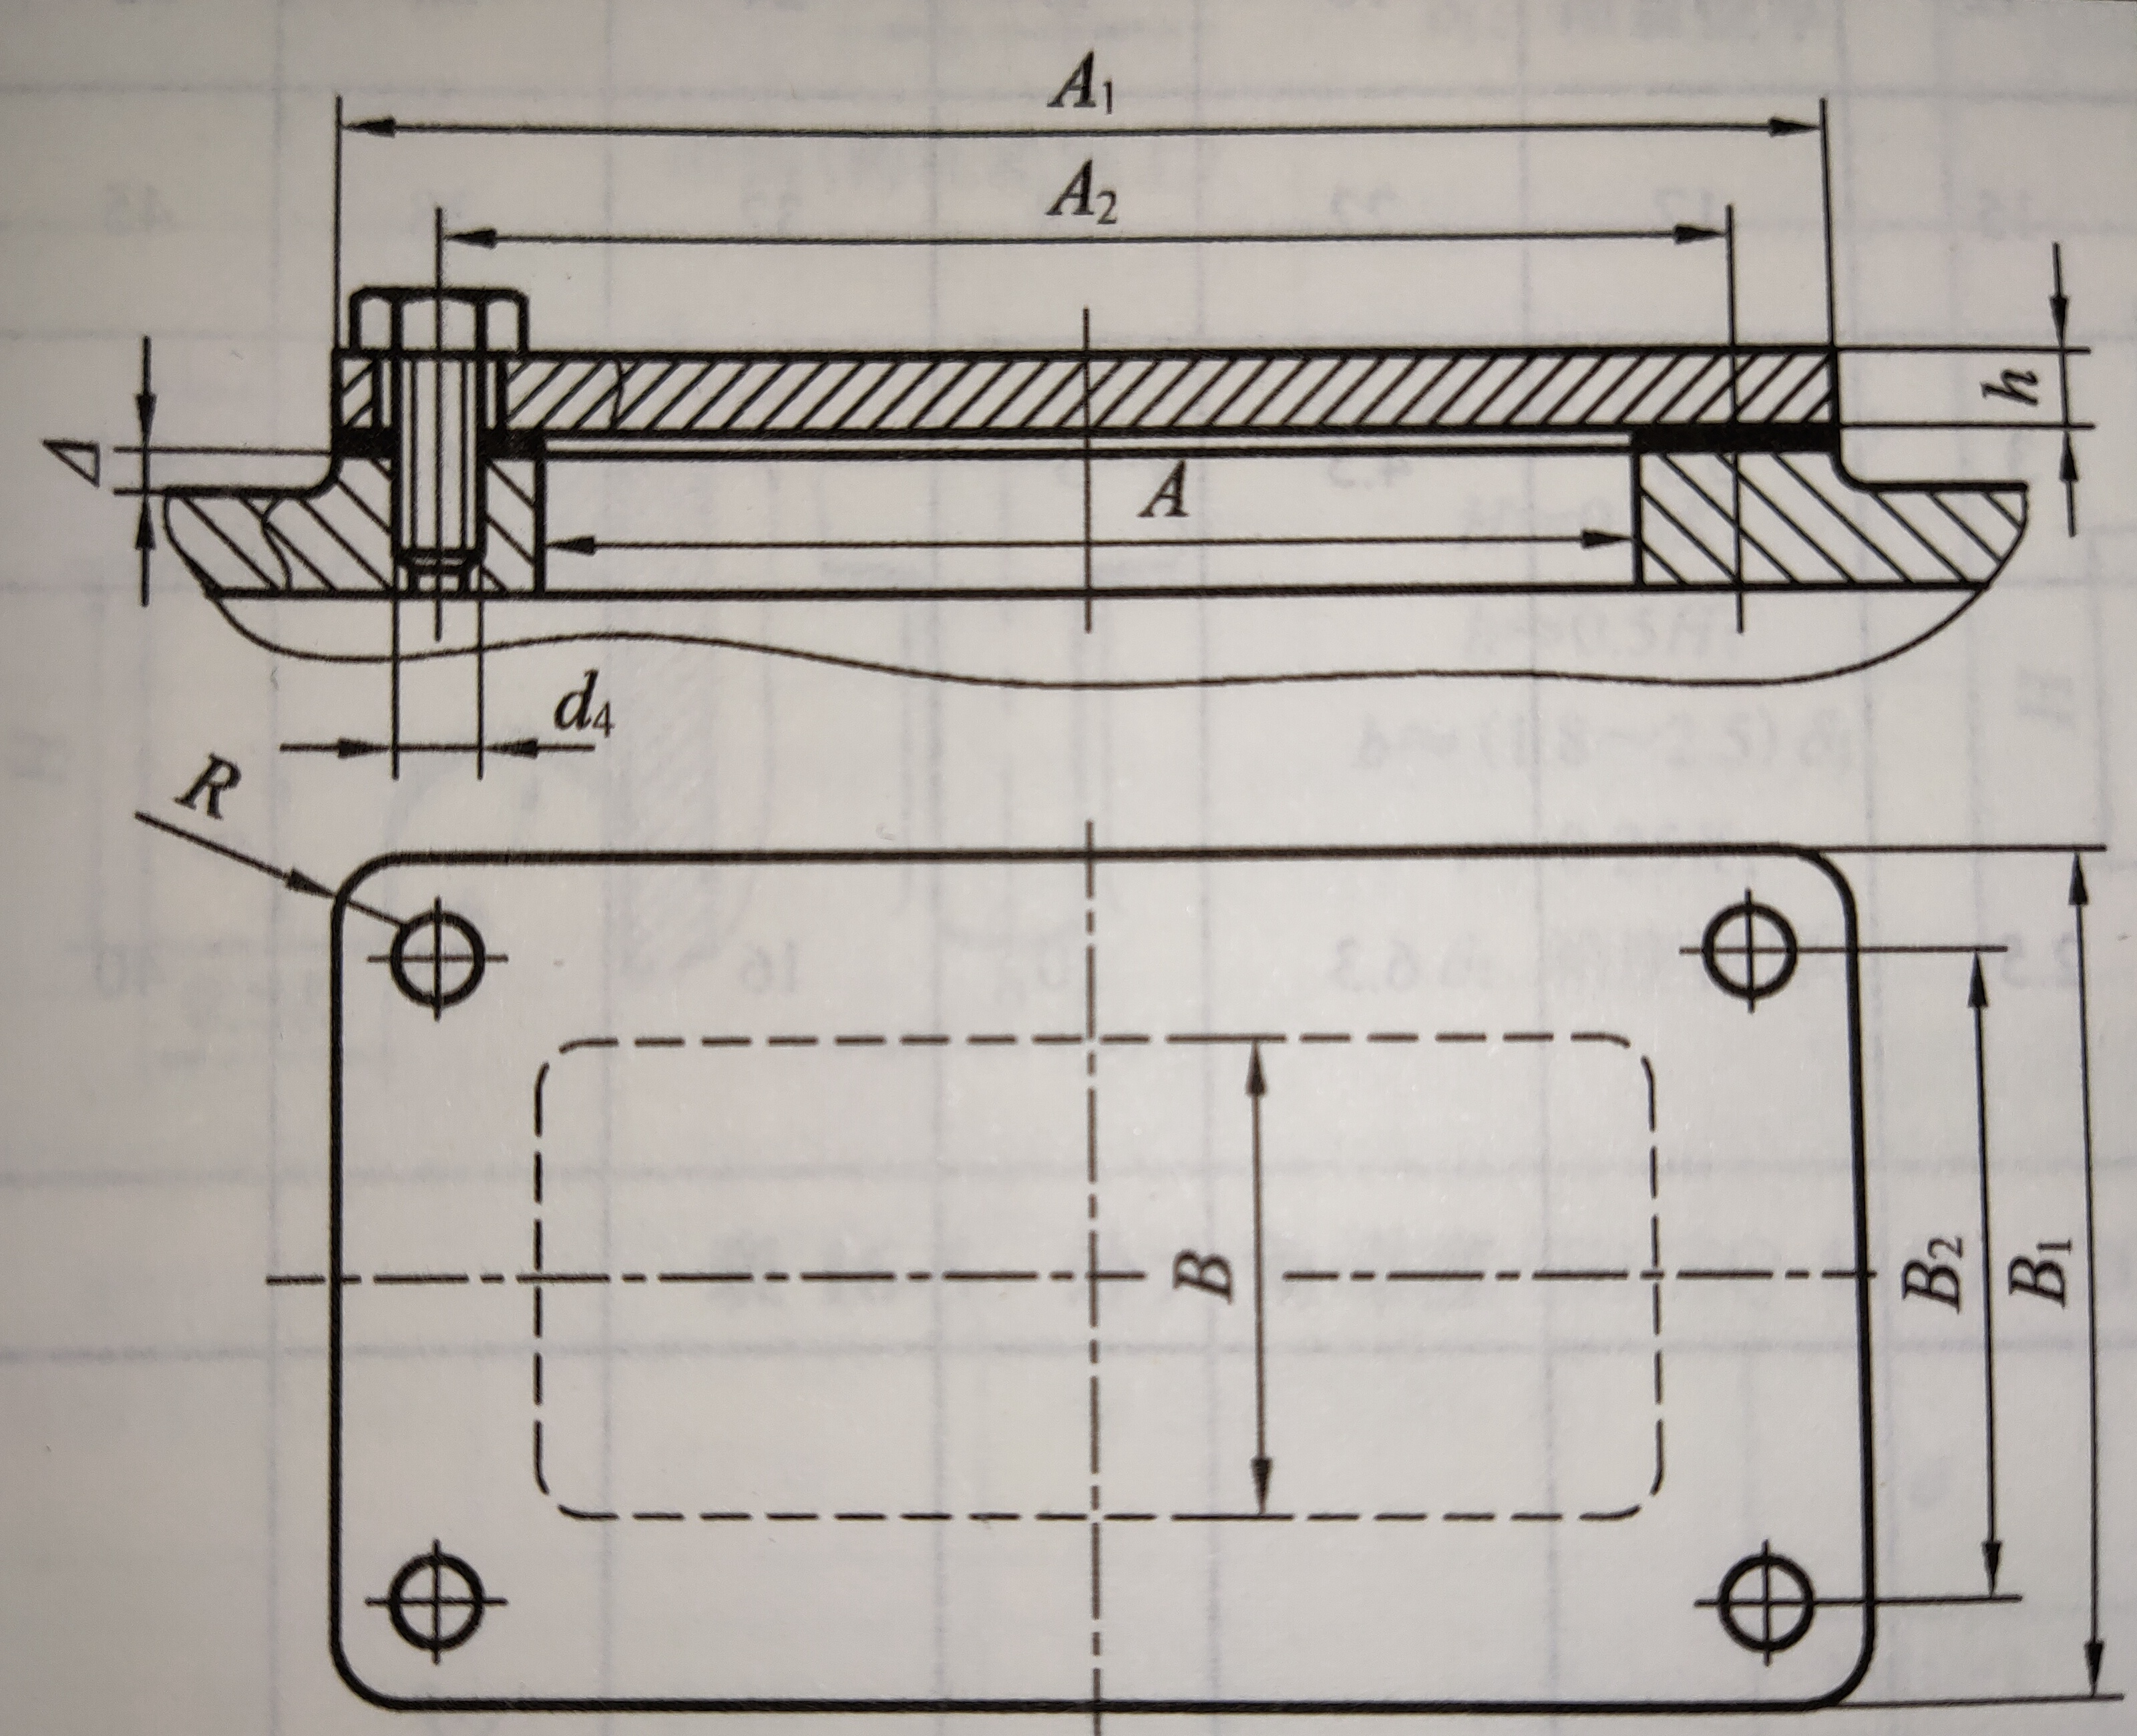
\includegraphics[scale=0.1]{graphic/10-1.jpg}
    \caption{轴的结构设计图检查孔和检查孔盖}
\end{figure}
查机械设计课程表$16-1$得具体尺寸如下:

$A=120mm,d_4=6mm,A1=A+5d_4=150mm,A_2=135mm,B_1=132mm$

$B=B_1-5d_4=102mm,B_2=117mm,R=6mm,H=3mm,\Delta=3mm$
\subsection{通气孔}
减速器工作,箱体内温度升高,气体膨胀,压力增大。通常在箱体顶部装设通气孔,使箱体内外压力平衡,不致使润滑油沿分箱面缝隙渗漏。垂直相通气孔的通气螺塞,其结构较为简单。若环境多尘可采用有滤网、防尘效果好的通气孔。

通气孔的主要尺寸设计如下:
\begin{figure}[h]
    \centering
    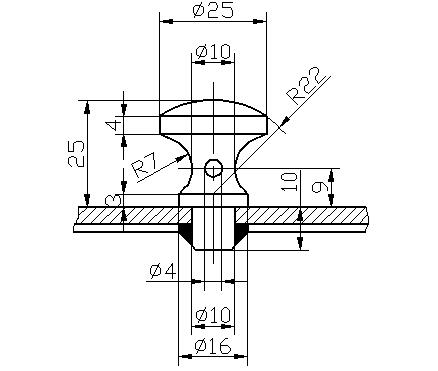
\includegraphics[scale=0.45]{graphic/10-2.jpg}
    \caption{通气孔}
\end{figure}
\subsection{定位销}
为了精确地加工轴承座孔,并保证每次拆装后轴承座的上下半孔始终保持制造加工时的位置精度,应在精加工轴承座前,在上箱盖和下箱盖的连接凸缘上配装定位销。采用的两定位圆锥销分别安置在箱体纵向和横向两侧的连接凸缘上,成非对称布置以加强定位效果。
\subsection{油面指示器}
用来指示箱体内油面的高度,油标位在便于观察减速器油面及油面稳定之处。油尺安置的部位不能太低,以防油进入油尺座孔二溢出。
\begin{figure}[h]
    \centering
    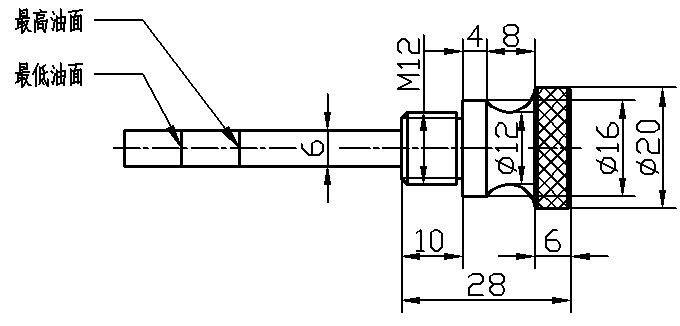
\includegraphics[scale=0.45]{graphic/10-5.jpg}
    \caption{油面指示器}
\end{figure}

\subsection{放油螺塞}
为排放减速器箱体内的污油和便于清洗箱体内部,在箱座油池的最低处设置放油孔,箱体内底面做成斜面,使油易于流出。
\begin{figure}[h]
    \centering
    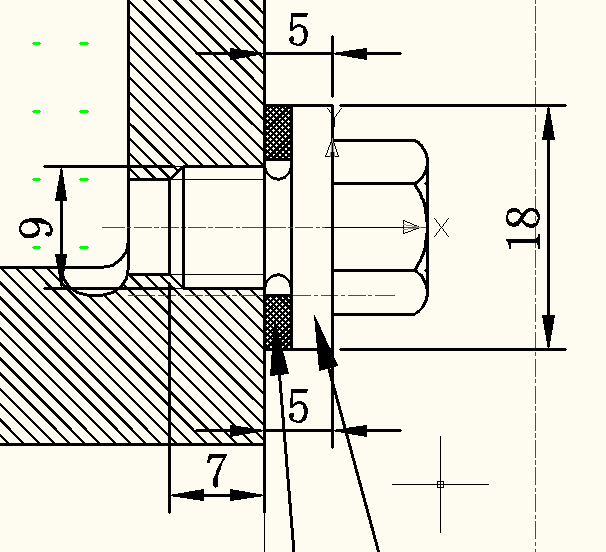
\includegraphics[scale=0.45]{graphic/10-6.png}
    \caption{放油螺塞}
\end{figure}

\subsection{起盖螺钉}
由于装配减速器时在箱体剖分面上涂有密封用的水玻璃或密封胶,因而在拆卸时往往因为胶结紧密难于开盖,旋动起盖螺钉可将箱盖顶起。选用的尺寸如图\ref{img4}

\begin{figure}[h]
    \centering
    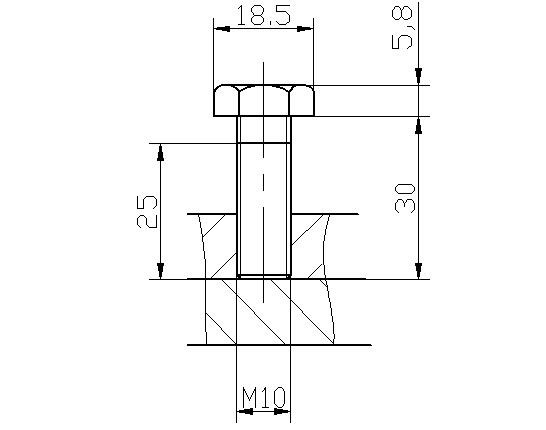
\includegraphics[scale=0.43]{graphic/10-4.jpg}
    \caption{起盖螺钉}
    \label{img4}
\end{figure}

\subsection{起吊装置}
起吊装置用于拆卸及搬运减速器。本设计采用吊环和吊耳。相关示例如\ref{img3}
\begin{figure}[h]
    \centering
    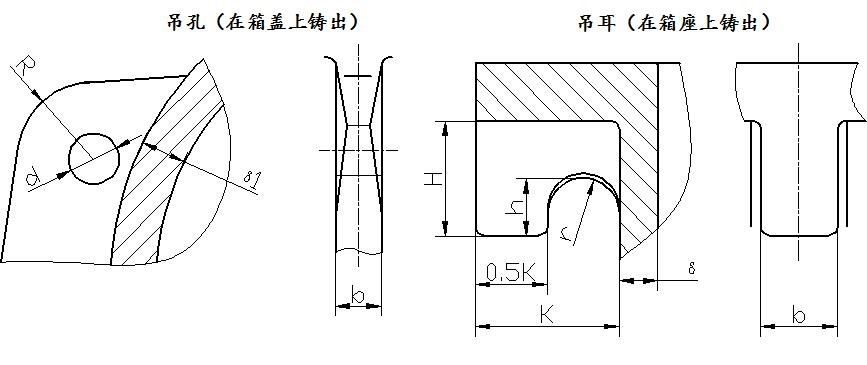
\includegraphics[scale=0.45]{graphic/10-3.jpg}
    \caption{起吊装置}
    \label{img3}
\end{figure}

吊孔尺寸计算
\[
b=2\delta_1=2\times 20=20mm
\]
\[
R= d=b=20mm
\]
\[
e=d=20mm
\]

吊耳尺寸计算

\[
K=C_1+C_2=20+16=36mm
\]
\[
H=0.8K=28.8mm
\]
\[
h=0.5H=14.4mm
\]
\[
r=0.25k=9mm
\]

    \section{设计小结}
课程设计是理论联系实际的一个过程。虽然只有短短的两个星期的时间,使我对机械设计这门课有了更深的理解和认识。机械设计的每一步都有它的理论支持,必须要按照它的标准进行。

作为一门基础学科,机械设计用到了之前学过的如工程图学、理论力学、材料力学、机械设计基础的内容。同时由于计算机技术的快速发展,计算机辅助设计也成为了机械设计工程不可缺少的技术。这次的机械设计中,我又通过复习了工程图学所讲述的CAD建模的知识,完成了零件和装配图的设计\cite{刘苏}。

最后,这次课程设计也离不开老师的悉心指导与帮助。在此衷心的感谢老师的指导与帮助。同时,由于时间短暂、知识的了解也不够充分,设计中会有一些不可避免的错误以及设计中未曾考虑到的缺点。如斜齿轮在正反转的过程中会有不同方向的轴向力,如何减少以至避免这个问题,还需要今后进一步的学习与思考,继续培养设计习惯和思维来提高实地操作的能力。

    %参考文献
	\kaishu
	\bibliographystyle{plain}
	\addcontentsline{toc}{section}{参考文献} %向目录中添加条目,以章/section的名义
	\bibliography{ref/main.bib}

\end{document}